%\documentclass[xcolor=dvipsnames]{beamer}
\documentclass[xcolor=dvipsnames, notes]{beamer}

\usetheme{Warsaw}

\usepackage{inputenc}
\usepackage{amsmath}
\usepackage{amsthm}
\usepackage{graphicx}
%\usepackage{geometry}
\usepackage{tasks}
\ifodd\textwidth
  \addtolength{\textwidth}{1sp}
\fi


\newcommand{\po}{\textcolor{BlueViolet}{po}}
\newcommand{\rf}{\textcolor{Green}{rf}}
\newcommand{\co}{\textcolor{BurntOrange}{co}}
\newcommand{\mo}{\textcolor{Red}{mo}}
\newcommand{\hb}{\textcolor{NavyBlue}{hb}}
\newcommand{\wb}{\textcolor{RoyalPurple}{wb}}
\newcommand{\hbsc}{\textcolor{NavyBlue}{hbsc}}
\newcommand{\fr}{\textcolor{RubineRed}{fr}}
\newcommand{\xhb}{\textcolor{NavyBlue}{xhb}}
\newcommand{\rfe}{\textcolor{Green}{rfe}}
\newcommand{\rfi}{\textcolor{Green}{rfi}}
\newcommand{\brf}{\textcolor{Green}{brf}}
\newcommand{\sw}{\textcolor{BurntOrange}{sw}}
\newcommand{\jhb}{\textcolor{NavyBlue}{jhb}}
\newcommand{\jmo}{\textcolor{Red}{jmo}}
\newcommand{\cf}{\textcolor{Apricot}{cf}}

\title{Formalizing the Concurrency Semantics of an LLVM Fragment}
\subtitle{Soham Chakraborty, Viktor Vafeiadis}

\author{Presented by \\ Akshay Gopalakrishnan}

\begin{document}
    
    \begin{frame}

        \maketitle
    \end{frame}

    %Summarize what the problem is
    \begin{frame}{Introduction}

        \begin{itemize}
            \item Compiler intermediate languages(IR) are useful for smoothly translating a source code to target, while also in the process exposing various performance based program transformations.
            \item While a lot of foundation has been built on the sequential semantics of such IRs, little formal work is done when translating concurrency semantics.
            \item In fact, most compiler IRs are too conservative in this aspect, thus not being able to perform certain aggressive transformations in this respect.
            \item Taking LLVM as an example, the concurrency (shared-memory) semantics is also specified informally, with suggestions for program transformations that should be (without formal proof) sound to perform. 
        \end{itemize}
        
    \end{frame}

    %Contributions of the paper.
    \begin{frame}{What the paper is about}

        \begin{itemize}
            \item Formal description of a fragment of LLVM concurrency semantics.
            \item Model axiomatic using Event Structures as opposed to per-candidate execution. 
            \item Proving standard theorems of Data Race Free (DRF).
            \item Proving soundness of compilation from C11 to proposed model of LLVM.
            \item Proving soundness of program transformations.
        \end{itemize}

    \end{frame}

    %Brief description of LLVM
    \begin{frame}{LLVM}

        \begin{itemize}
            \item An intermediate representation(IR) for C/C11 programming language (rudimentary support for Java).
            \item As an IR, it also has its own concurrency model to support program analysis and optimizations.
            \item List of transformations it performs is the most valuable part of the specification.
            \item However, its concurrency model is informal and in relative prose format, thus not able to make use of program transformations to the fullest (eg: Redundant elimination). 
        \end{itemize}

    \end{frame}

    %Undefined value semantics.
    \begin{frame}{Notion of Undefined Value}

        LLVM assigns a read an undefined value $u$ if required.
        This can happen, if the read value is possible to return any random value (eg: Uninitialized value).
        The properties of this value $u$ are:
        \begin{itemize}
            \item $u+1=u$
            \item $u*v=v$ ($v$ is some defined value).
            \item $u*0=u$
            \item .... and so on.
        \end{itemize}
        
    \end{frame}

    \begin{frame}{Example: Sequential}

        %Add sequential example here to potray implications of undefined value.
        \begin{figure}
            \makebox[\textwidth][c]{
                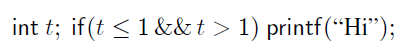
\includegraphics[scale=0.7]{EX_SEQ.PNG}
            }
        \end{figure}

        The above program can print the text "Hi" as variable "t" is Uninitialized and hence its read will be assigned undefined value $u$.

    \end{frame}

    \begin{frame}{Implications in Concurrency - Program Transformations}

        In C11, any program with data races has undefined behavior.
        This means, some read value is non-deterministic and hence can be assigned as per LLVM value $u$.
        
        This semantics is stronger than that of C11, which declares data race programs to have undefined behavior.

    \end{frame}

    \begin{frame}{Example: Concurrent}

        %Add the concurrency C example here to show how undefined behavior would be taken advantage of.
        \begin{figure}
            \makebox[\textwidth][c]{
                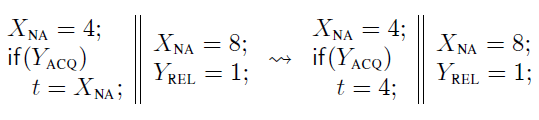
\includegraphics[scale=0.7]{EX_CONCUR.PNG}
            }
        \end{figure}

        The above Transformation is possible only because the two writes to $X$ are in a race.
        In terms of LLVM, the read value will be undefined $u$.
        Then the above Transformation could be applied, giving the read any appropriate value (in this case $4$).
    
    \end{frame}

%-----------------------------------------------------------------------------------------------------------------------------------------

    %Prime event structures and Memory Event Structures.
    \begin{frame}{LLVM Formalization: Event Structures}

        Prime event structure.
        Consists of 
        \begin{itemize}
            \item Events of a program ($V$). 
            \item Program order ({\po}) defining intrathread syntactic order. 
            \item Conflict relation ({\cf}), relating events and also implying thread executions that can never occur together.
        \end{itemize}
        Memory event structure.
        \begin{itemize}
            \item Prime event structure.
            \item Reads-from relation ({\rf}) relates every read to the write from which its value comes from.
        \end{itemize}
        
    \end{frame}

    \begin{frame}{LLVM Formalization: Auxilary Definitions}
    
        \begin{itemize}
            \item Race(G) : Two events race if at least one of them is a write and at least one of them is non-atomic.
            \item WWRace(G) : Checks if event structure has race between two writes.
            \item hbW(e) : Checks if read event $e$ has some write which is initialized that it can read from. 
            \item AddRF(G,e,e') : Creates an {\rf} edge between two events in an event structure.
            \item locs : $(e,e') \| loc(e) = loc(e')$.
        \end{itemize}
        
        %We may have to even put event orders here. Perhaps we should.
        %Event orders.

    \end{frame}

    \begin{frame}{LLVM Formalization: Auxilary Definitions}
        
        Access orders/modes
        \begin{figure}
            \makebox[\textwidth][c]{
                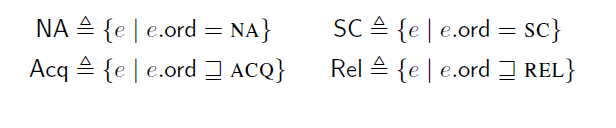
\includegraphics[scale=0.7]{AUX_DEF_ORDERS.PNG}
            }
        \end{figure}

        \begin{itemize}
            \item Synchronize with ({\sw}): $[Rel];\rf;[Acq]$. 
            \item Happens before ({\hb}): $(\po \cup \sw)^{+}$.
        \end{itemize}

    \end{frame}

    \begin{frame}{LLVM Formalization: Event Structure Building Rules}
        
        \begin{figure}
            \makebox[\textwidth][c]{
                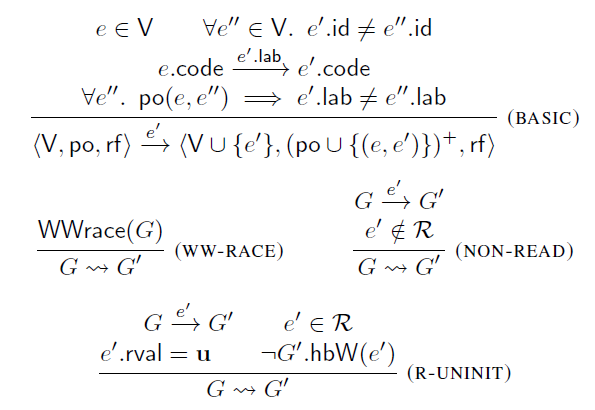
\includegraphics[scale=0.7]{EVENT_STRUCTURE_RULES1.PNG}
            }
        \end{figure}

        \begin{figure}
            \makebox[\textwidth][c]{
                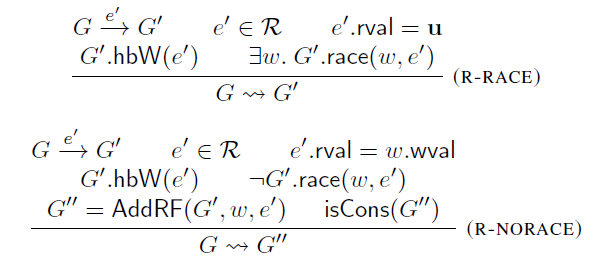
\includegraphics[scale=0.7]{EVENT_STRUCTURE_RULES2.PNG}
            }
        \end{figure}

    \end{frame}

    \begin{frame}{LLVM Formalization: Event Structure Construction}
        
        Consider an event structure $G$.
        \begin{itemize}
            \item Pick an event not in the current event structure (BASIC).
            \item This event should be {\po} after(if exists a po relation) events in an event structure (BASIC).
            \item If this is a write, just add this to event (NON-READ).
            \item If this is a read, then we also add a reads-from relation using AddRF if no race otherwise just add $u$ (R-UNINIT, R-RACE, R-NORACE).
        \end{itemize}
        
    \end{frame}

%--------------------------------------------------------------------------------------------------------------------------------------------

    \begin{frame}{LLVM Formalization: Consistency Rules}
        
        \begin{itemize}
            \item Overwritten writes >> W-W'-R.
            \item Conflicting writes >> Writes on conflicting branches cannot satisfy reads.
            \item Non-Conflicting Justifications >> Conflicting writes cannot justify non-conflicting reads (cuz the program would then have OOTA behavior).
            \item Preserving order of SC accesses.
        \end{itemize}
        
    \end{frame}

    \begin{frame}{Overwritten Writes}
        
        We want to disallow reads from reading write values that were clearly overwritten. 
        For this, we have the \textit{writes before} relation.
        %Show its definition here
        \begin{align*}
            \wb = [W];((\brf;((\hb \cap locs);\brf) \text{ \textbackslash} \brf);[W]).
        \end{align*}

        We require {\wb} to be irreflexive, thus ensuring overwritten writes are properly ordered. 
    \end{frame}

    \note{
        The intuition behind the writes before definition is the following:
        \begin{itemize}
            \item Firstly, we need to order the writes in a program.
            \item But we mainly need to only order the writes which are read from (we are talking about execution graphs). 
            \item It is only among these writes that conflict might occur, as reads-from relations would imply some order between writes.
            \item Also, the conflict may occur only between writes both of which can be read from.
            \item The {\brf} basically collects also the writes having reads-from relations.
            \item The {\wb} then only takes those writes ordered by {\hb}.
            \item Thus, you could say {\wb} is a subset of {\hb} restricted to writes which are definitely read from some read in the program.
        \end{itemize}
    }

    \begin{frame}{Conflicting Writes}

        If a read is justified by a write it conflicts, then it is also an incorrect execution. 
        More generally, {\hb} related events must not be in conflict. %This might be a bit confusing as rf relations may then be established without {\hb} edges too.
        So we require {\cf;\hb} to be irreflexive.
        
    \end{frame}

    \note{
        As far as the model in the paper goes of LLVM, reads are either non-atomic, acquire or SC.
        In C11, it is required that non-atomic read values only come from writes that happen before it. Whereas the release and SC reads, while forming a reads-from relation, also imply a happens-before relation. Since LLVM closely resembles (except for the Data Race condition) C11 model, the above irreflexivity condition will suffice.
    }

    \begin{frame}{Non-Conflicting Justifications}

        If a program has reads justified by writes which conflict, then even such executions are incorrect. 
        More specifically, we want to disallow cases reminiscent of Out-of-Thin-Air behaviors.
        For this, we disallow writes to justify non-conflicting {\hb} related reads.
        The authors frame this requirement as ${\rf;\hb^{-1};\rf^{-1};\cf}$ to be irreflexive.

    \end{frame}

    \note{
        The intuition behind the above irreflexivity relation is as follows:
        \begin{itemize}
            \item We want to ensure that conflicting writes do not justify non-conflicting {\hb} related reads.
            \item So firstly we do not want $[W];\cf;[W]$ to be having reads-from relations with non-conflicting reads.
            \item For this, we first connect the first write with some read that reads from it (\rf).
            \item Then we trace back happens before, reaching another read. ($\rf;\hb^{-1};[R]$).
            \item Then we connect this read to its read-value ($\rf;\hb^{-1};\rf^{-1}$).
            \item Now this write should not be in conflict with the initial one, thus giving us $\rf;\hb^{-1};\rf^{-1};\cf$ to be irreflexive. 
        \end{itemize}
    }


    \begin{frame}{Preserving Order of SC Accesses}

        \begin{itemize} 
            \item Not relying on official C11 model's definition as it is flawed, in that several architecture compilation schemes are unsound.
            \item Instead, rely on the SC definition in RC11 paper (Lahav et.al.)
            \item This requires a union of relations to be acyclic.
        \end{itemize}
        
    \end{frame}
    
    \note{
        To understand intuition on the new SC definition, one would need to read the RC11 paper in detail. 
        Also, I am unsure of why the definition of SC in C11 is flawed. This is also mentioned using counter example in the RC11 paper. 
        So to understand better the definition, one must go into that.
    }

    \begin{frame}{Preserving Order of SC Accesses}
        
        Basic definitions:
        \begin{itemize}
            \item Read-before (${\fr}$) : $\rf^{-1};\wb \text{\textbackslash} [V]$.
            \item Program location based order (${\po_{locs}}$) : $\po \text{\textbackslash} locs$.
            \item Happens-before-SC (${\hbsc}$) : $[SC];((\hb \cap locs) \cup (\po_{|\neq locs}) \cup (\po_{|\neq locs};\hb;\po_{|\neq locs}));[SC]$
        \end{itemize}
    
        The axiom for preserving SC then requires $(\hbsc \cup \wb \cup \fr);[SC]$ to be acyclic.

    \end{frame}

    \note{
        I am unsure why instead of relying on a modification of the original SC definition $(\po \cup \rf \cup \mo \cup \fr)$ acyclic, the authors have, or rather the RC11 paper has adopted to have these new definitions.
        Maybe there is an obvious connection, which I am unable to decipher at this point of my understanding. 
    }

    \begin{frame}{Consistent Event Strucutre and Observable Behavior}

        To summarize an event structure is consistent if the following hold:
        \begin{figure}
            \makebox[\textwidth][c]{
                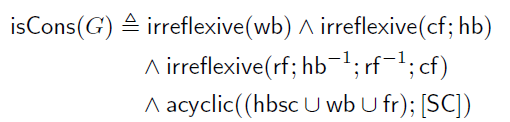
\includegraphics[scale=0.7]{CONSISTENT_EVENT_STRUCTURE.PNG}
            }
        \end{figure}

        Further, an observable behavior of an event structure is the set of last write values written to memory.
        That is:
        \begin{align*}
            Behavior(G) = \{(l,v)| \exists e \in G.V. \ v \leq e.wval \ \wedge \ \nexists e'. \ G.wb(e,e')\} 
        \end{align*}

    \end{frame}

    \note{
        Its interesting to see that observable behavior has this definition, in contrast to being the read values a program gives in any execution.
        This allows you, as Soham mentioned, reason about programs without even having any read accesses in them. 
        This is better.
    }

%---------------------------------------------------------------------------------------------------------------------------------------
    %DRF Theorems
    \begin{frame}{DRF Theorems}

        The above model respects the following DRF Guarantees.
        \begin{itemize}
            \item \textbf{DRF-RA}: \textit{If under RA Consistency a program has no read-write races, then its LLVM consistent behaviors coincide with RA-Consistent ones.}
            \item \textbf{DRF-OSC}: \textit{If a program is RA race-free under OSC, then OSC and LLVM consistency coincide.}
        \end{itemize}

    \end{frame}

    \begin{frame}{DRF-RA Proof Elements}

        \begin{lemma}{Lemma 1}
            \tag{Lemma1}
            If an LLVM consistent event structure $G$ has no read-write races, then $G$ is also RA consistent.  
        \end{lemma}

        \begin{lemma}{Lemma 2}
            \tag{Lemma2}
            Given a program $P$ and LLVM-consistent event structure of $P$ with a read-write race, there exists some RA-consistent event structure of $P$ with a read-write race.
        \end{lemma}
    
    \end{frame}

    \note{
        TODO
    }

    \begin{frame}{Proof}

        DRF-RA, formally stated:
        \begin{align*}
            [P]_{RA} \ \wedge \ \neg RWRace_{RA}(P) \ \Rightarrow \ [[P]]_{RA} \ = \ [[P]]_{LLVM}. 
        \end{align*}

        To prove this, we need to show:
        \begin{align*}
            [[P]]_{RA} \ \subseteq \ [[P]]_{LLVM} \\
            [[P]]_{LLVM} \ \subseteq \ [[P]]_{RA}
        \end{align*}

    \end{frame}

    \begin{frame}{Proof cnt'd}
        The first case holds trivially, as by definition LLVM model is stronger than RA.

        For the second case, divide into the following two cases for every event structure $G$ of $P$:
        \begin{align*}
            Cons_{LLVM}(G) \ \wedge \ \neg RWRace_{LLVM}(G).\\
            Cons_{LLVM}(G) \ \wedge \  RWRace_{LLVM}(G).  
        \end{align*}

        The first case, if so, by Lemma \ref{Lemma1} guarantees that $G$ is also RA-Consistent.
        The second case, if so, by Lemma \ref{Lemma2} guarantees that $G$ is also RA-Consistent and has a read-write race, which contradicts our assumption that $P$ has no read-write races under RA.

        Hence proved.
    \end{frame}

    \note{
        TODO
    }

    \begin{frame}{DRF-OSC Preliminary definitions}

        \begin{itemize}
            \item RARace: $\exists a,b \in G.V \ . \ a.loc=b.loc \ \wedge \ \neg(a.ord=SC \wedge b.ord=SC) \ \wedge \ (a \in W \vee b \in W)$.
            \item Observable Sequential Consistency : SC without the WW-Race rule for constructing event structure. Only {\wb} relation is used to order writes. 
        \end{itemize}

    \end{frame}
        

    \begin{frame}{DRF-OSC Proof elements}

        \begin{lemma}{Lemma 3}
            If an RA-consistent event structure $G$ is RA-race free, then $G$ is also OSC-consistent. 
        \end{lemma}

        \begin{lemma}{Lemma 4}
            For every RA-racy LLVM-consistent event structure, there exists an RA-racy OSC-consistent event structure.
        \end{lemma}

    \end{frame}

    \note{
        Proof of Lemma 3 is not well written in the appendix.
        Firstly, RWRace is contained in RARace. 
        This means, by Theorem 1, RA-consistent coincides with LLVM consistent one.
        So our Lemma then requires us to just prove LLVM-consistent without RA-race(since behaviors coincide, it also means orders between events, hence no RARace too) is also OSC-Consistent.
        This the authors prove by contradiction.
        If it isn't OSC-consistent, then there is a read which reads from some old write (which also means no other write $w'$ is {\hb} before this read).
        Two cases for this, both the read and write are SC, which by construction then make it trivially OSC.
        If both not SC, then they should be in an RARace by definition, but by our assumption this is not true.
        Hence proved. (poorly written proof but whatever)
        Lemma 4 is proved by constructing event structure from point where no races exist. 
        The step which causes a race is also OSC-consistent and has an RARace. 
    }

    %Keep this bit very straightforward.
    \begin{frame}{Proof Intuition}

        DRF-OSC formally stated:
        \begin{align*}
            \forall P.DRF_{OSC}(P) \ \implies \ [[P]]_{LLVM} = [[P]]_{RA} = [[P]]_{OSC}. 
        \end{align*}

        Note that the RARace definition here corresponds to the same function $DRF_{SC}$ that we use above.
        Note also that we get $[[P]]_{RA}$ here as its usage in the above lemmas will help us prove this theorem.
        Proof of the above statement is in two parts:
        \begin{itemize}
            \item $\forall P.DRF_{OSC}(P) \ \implies \ [[P]]_{LLVM} = [[P]]_{RA}$.
            \item $\forall P.DRF_{OSC}(P) \ \implies \ [[P]]_{LLVM} = [[P]]_{OSC}$.
        \end{itemize}

    \end{frame}

    \note {
        The fact that we get RA consistent programs too in the picture is kind of ingenious to me.
        Is it possible to prove this without involving release acquire?
        If not, how did the authors figure out that RA consistency as an intermediate step would be the solution?
        This only tells me that I have yet to learn from my own experience working with proofs.
    }

    \begin{frame}{Proof Intuition cnt'd}

        The first case can be proven directly using $DRF-RA$ theorem proven before.
        Because $DRF_SC$ contains $RWDRF_{RA}$.

        The second case can be proven because we have 
        \begin{align*}
            \forall G \in P. \neg RARace(G).
        \end{align*}
        By Lemma 3, we have then $[[P]]_{RA} = [[P]]_{OSC}$ and by the first case proven, we can infer by transitivity $[[P]]_{LLVM} = [[P]]_{OSC}$.
        
    \end{frame}

    \note{
        The above proof is slightly different from the original. 
        The actual proof considers two cases to prove, firstly LLVM subset of OSC and vice versa.
        I found this a bit confusing, as we already have that RARace does not exist in the program, thus every RA-consistent is also OSC-Consistent as per Lemma 3. 
        Need to investigate their reasoning better (perhaps ask viktor or soham?).
    }


    %Compilation from C11 to LLVM
    \begin{frame}{From C11 to Proposed LLVM model}

        Since the semantics are the same except that regarding data races, it suffices to show that undefined behavior of C11 contains that of LLVM read values having value $u$.
        So the following:
        \begin{align*}
            [[P]]_{LLVM} \ \subseteq \ [[P]]_{C11}.
        \end{align*}
        is trivial as undefined behavior can contain another undefined behavior. 
        
        Note that the above is assuming the SC axioms are the new ones proposed in RC11 for C11.

    \end{frame}

    % Transformations 
    \begin{frame}{Validity of Program Transformations}

        The transformations considered are:
        \begin{itemize}
            \item Reordering of independent accesses.
            \item Elimination of reads.
            \item Strengthening of accesses.
            \item Introduction of reads.
        \end{itemize}

        Note also that the following must hold for any valid transformation:
        \begin{align*}
            P_{src} \mapsto P_{trnsf} \ \Rightarrow \ [[P]]_{trsf} \subseteq [[P]]_{src}.
        \end{align*}
    \end{frame}

    \begin{frame}{Reordering}
        The proof for this is done using induction and constructing event structures for both programs. 
        Firstly, note that because we have multiple event structures, we have to reason about the soundness in all of them.
        For this, firstly, we set up event structure such that the sets of one-to-one {\po} relations for both programs are same. 
        Then, we follow for each a different path (based on the reordering) and then collapse the event set to represent the desired event structure.
        The crux is that there will always be a way to collapse to find an event structure for both programs representing the same behavior.
    \end{frame}

    \note{This can be done using our thesis idea, where we ensure that equality of sets remain ({\po} or {\hb}).
    Because of this, the behaviors in the transformed programs will be contained in that of the source.
    The axioms/ consistency rules will ensure that read values either come from racy writes or one that respects coherence. 
    Since we add more {\hb} relations by reordering, the set of behaviors will trivially be a subset of the source program.}

    \begin{frame}{Elimination}
        Three forms of elimination are considered:
        \begin{itemize}
            \item Overwritten Write (OW) - $x=1;x=2; \ \mapsto \ x=2;$. - 
            \item Read After Write (RAW) - $x=1;a=x; \ \mapsto \ x=1;$.
            \item Read After Read (RAR) -  $a=x;b=x; \ \mapsto \ a=x;$
        \end{itemize}

        Note that the eliminated event in the above transformation is only those that are non-atomic.
        The proof for each of this transformation is done by considering one single event structure step in target program to be a two event addition step in the source program.
        This shows that behaviors in transformed program can be reproduced in the source.

    \end{frame}

    \begin{frame}{Strengthening}
        This involves modifying the type of the access such that for the current type $o$ and modified type $o'$, the latter is stronger ($o \subset o'$).
        The proof for this is straightforward as LLVM model respects monotonicity, which requires that:
        \begin{align*}
            P \Longrightarrow P'_{strong} \ \Rightarrow \ [[P']] \subseteq [[P]].
        \end{align*}
    \end{frame}

    \note{
        The above proof can be done by showing that any event structure consistent in $P'$ has an equivalent event structure in $P$.
        The strengthening of accesses would mean at teh very least, non-atomic to be release/acquire/SC. In either case, we will have more {\hb} relations, which inevitably means lesser behaviors and they are included in the source program's set of behaviors.
        }

    \begin{frame}{Introduction}

        Here, only load introduction is considered. 
        Note that in C11, such a transformation is unsound as it may lead to data races, thus giving a program potentially undefined behavior.
        However, in LLVM such a transformation is frequently performed.
        %Not sure whether it can be proven sound in LLVM due to the undefined value $u$. 
        %Proof or counter example not present in the paper/appendix.

    \end{frame}

    %Compilation to Hardware (x86-TSO)
    \begin{frame}{From LLVM to x86-TSO}
        The mapping from LLVM model proposed to x86-TSO is proven to be sound.
        This is implied directly due to DRF-RA based results.
        The proof intuition is as follows:
        \begin{itemize}
            \item We know that for every LLVM racy execution, we have a racy execution in RA.
            \item We also know that for every LLVM program with no races, it implies program in RA has no races.
            \item From monotonicity property, the mapping of accesses from LLVM to x86-TSO makes all weaker accesses to either release or acquire (SC will be followed by an MFENCE).
            \item Now since all accesses are atomic, we have no races. Thus by DRF-RA, the behaviors under LLVM coincide with RA.
            \item Using existing result of RA to x86-TSO mapping being correct, the proof follows by simply transitivity. 
        \end{itemize}

    \end{frame}

    \note{
        The proof of mapping from RA to TSO is similar to the proof we have written for TSO to SC.
        Proof by contradiction is the trivial way to do it.
    }

    \begin{frame}{Thank you}

        Questions?

    \end{frame}


\end{document}

